\chapter{Règles de changement d’états et moteur de jeu}

\section{Règles de changement d’états}

Le tour de jeu d’un joueur est terminé lorsque tous ses personnages possèdent un statut USED ou DEFENDING.
\\Les actions sont réalisées en fin de tour dans l'ordre entré par le joueur actif. 
C’est alors le tour du joueur adverse.
\\Lorsqu’un personnage est attaqué par un ennemi, il perd des points de vies correspondant à 
l'attaque de l'attaquant moins sa défense.
Lorsqu’un personnage utilise un objet, il peut l'utiliser sur lui-même ou sur 
un autre personnage, pour gagner des points de vie par exemple.
\\Si un personnage perd tous ses points de vie, son statut évolue et prend la valeur DEAD.
Si tous les personnages d’un joueur meurent, la partie est terminée 
à la fin du tour et le joueur adverse gagne.
\\Chaque action effectuée modifie l’état des personnages concernés, 
autant celui la réalisant que les victimes. 
Le choix du personnage sélectionné et des actions effectuées est provoqué par des commandes.
Pour ce jalon une séquence de commande est réalisée dans le fichier "main.cpp".
\\Le scénario de test comporte 5 tours, on peut jouer un tour en appuyant sur la touche E.


\section{Conception logicielle}
Le diagramme des classes UML C++ pour le moteur est visible en Figure 4.1.
On divise le moteur de jeu en 3 groupes de classes.
\begin{itemize}
    \item \textbf{Le agroupe de la classe Engine:} C’est le coeur du moteur du jeu. 
    Cette classe permet de stocker les commandes dans un vecteur de Command (avec l'opération "addCommand"). 
    Ce mode de stockage permet d’introduire une notion d'ordre: on réalisé les commandes dans 
    l'ordre où le joueur les à rentrées. Lorsque turnCheckOut est appelé les commandes sont exécutées, 
    si tout les personnages ont des actions ou s'ils passent leur tour, puis on change de joueur actif.
    \\
    \item \textbf{Le groupe de la classe Command:} C'est la classe maîtresse des actions. 
    Elle définie les méthodes de manière abstraite afin quelles soient utilisables et 
    modifiables par toutes les actions grâce au polimorphisme.
    \\
    \item \textbf{Le groupe des classes Attack, Defend, Move, EndTurn, UseObject et UseSkill:} 
    Les classes Attack, Defend, Move, EndTurn, UseObject et UseSkill, héritant de la classe
    Command, possèdent chacune une méthode "validate" qui permet de savoir si le personnage et 
    capable de réalisé la commande et une méthode "action" qui fait exécuté au personnage 
    l’action correspondante à la commande. Chacun possède aussi un constructeur permettant de 
    savoir quel personnage réalise l'action, quel(s) personnage subit l'action et les spécificités 
    liées à chacune des actions.
\end{itemize}



\begin{figure}[H]
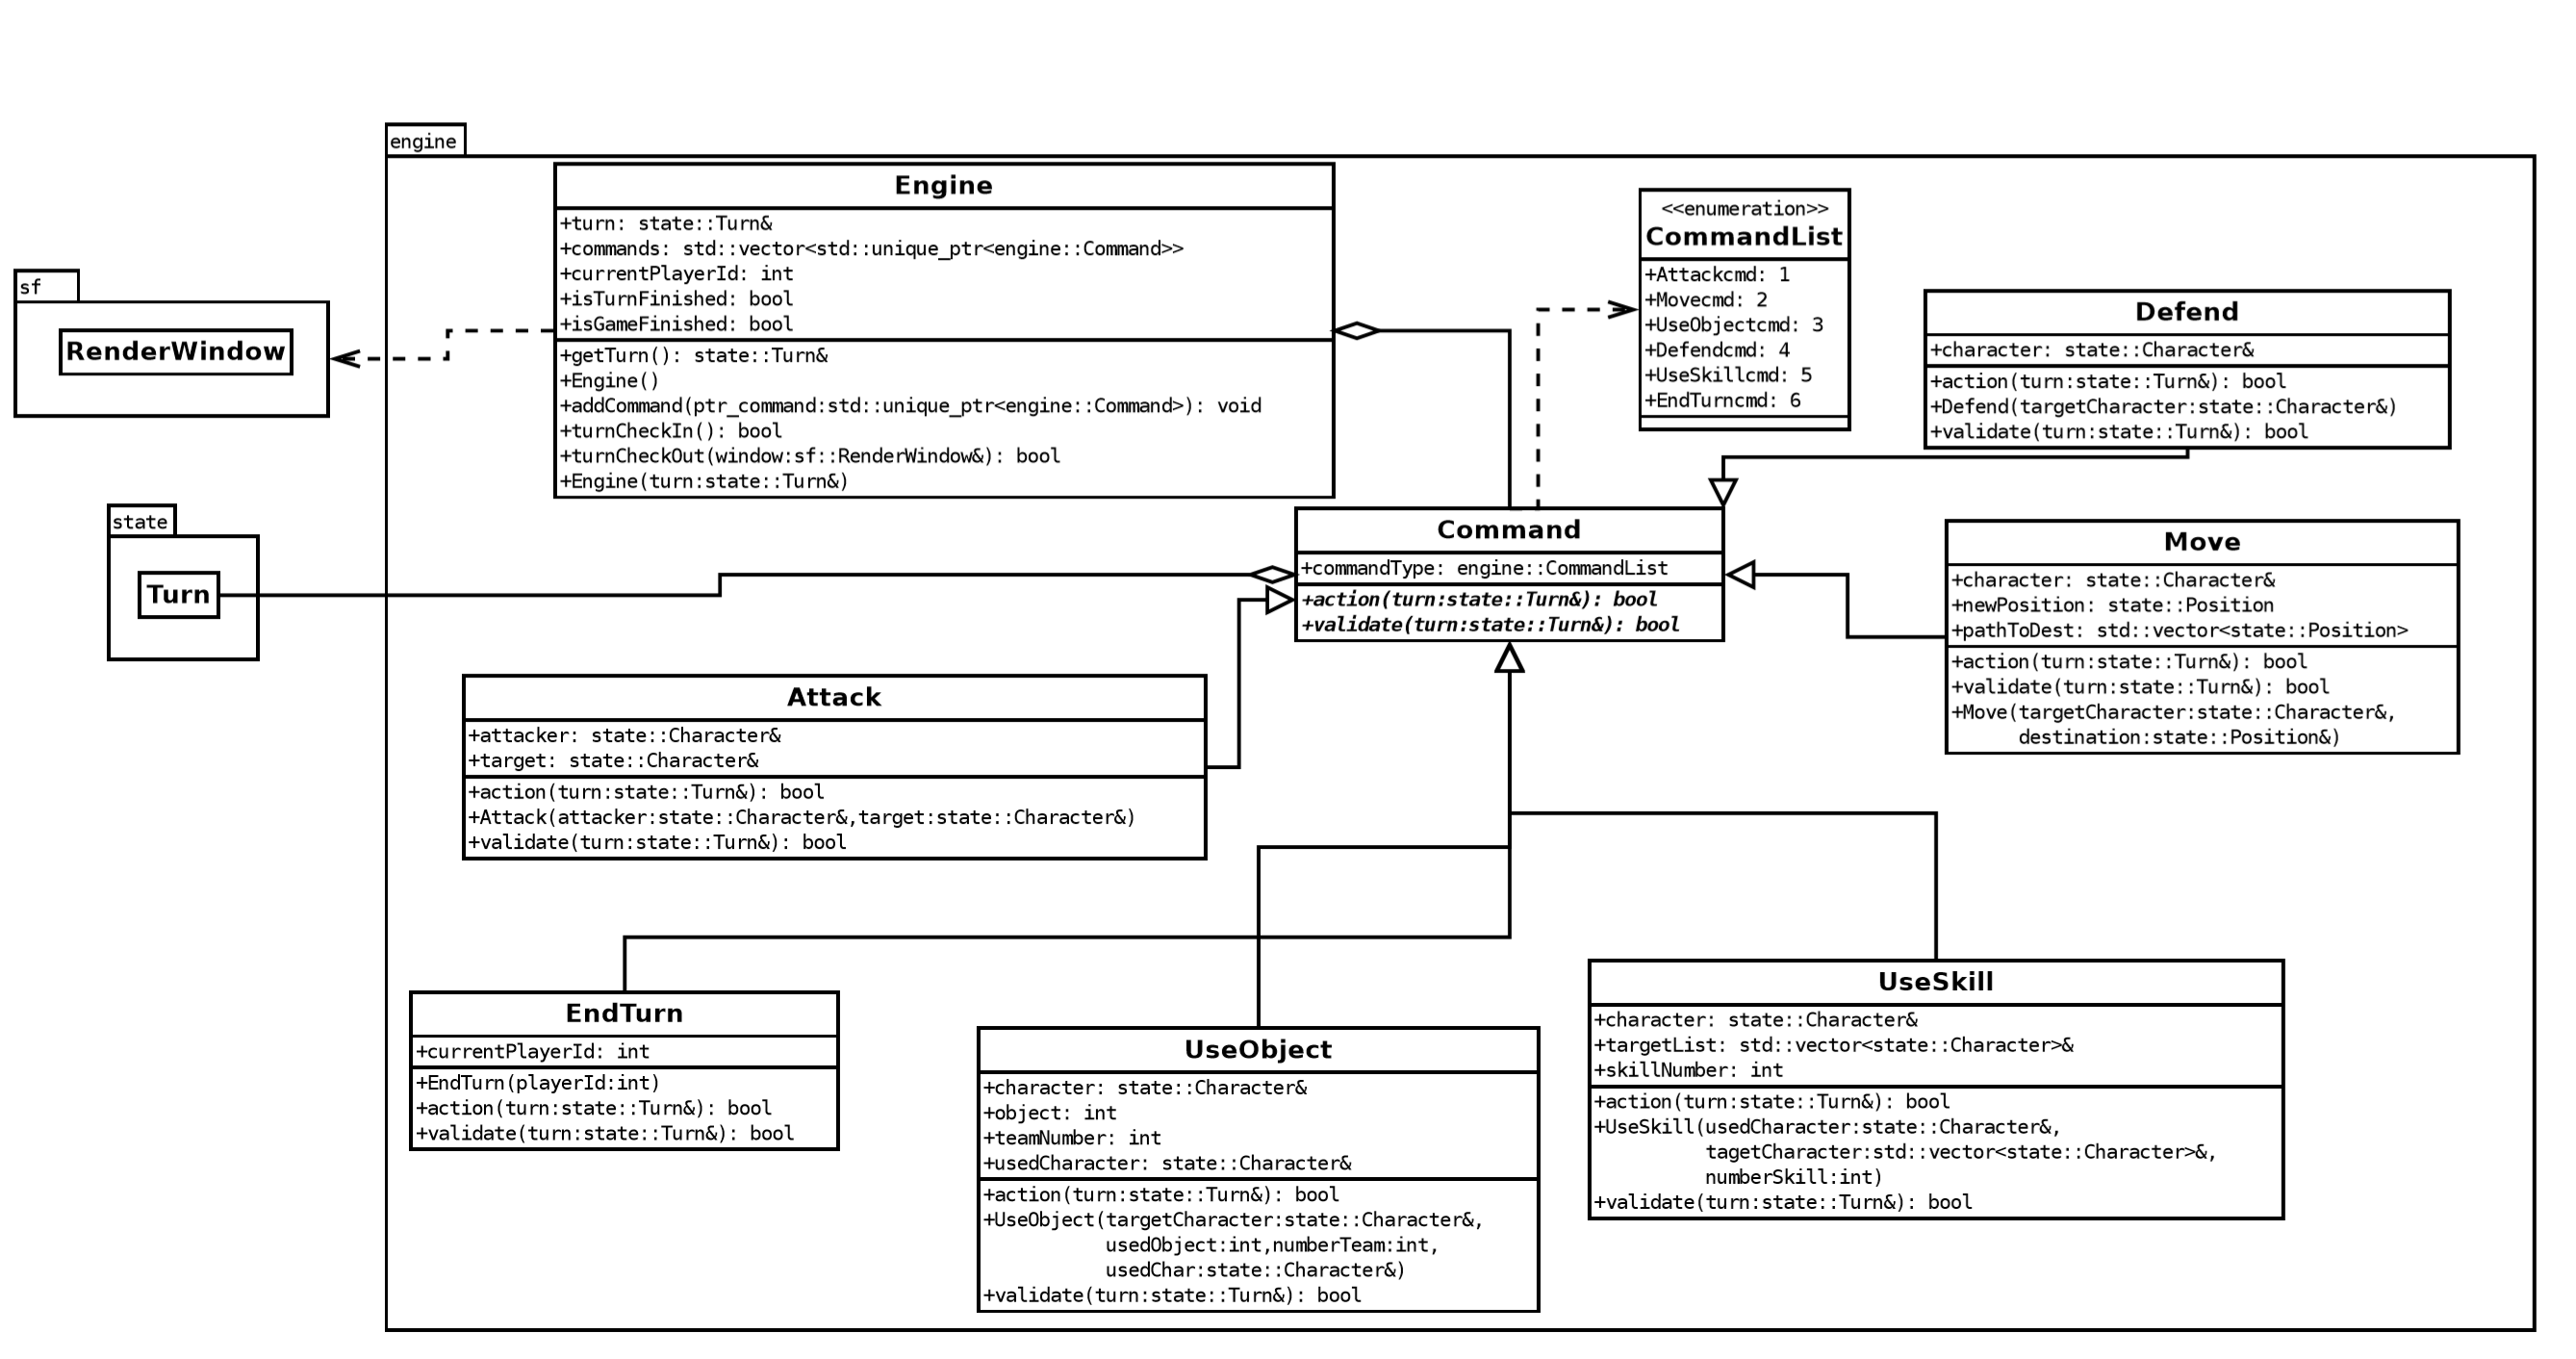
\includegraphics[width=\linewidth]{images/engine_dia.png}
\centering
\caption{Aperçu de engine.dia}
\label{fig:img3}
\end{figure}
